\scanpage{154}
% archive foliation: 153
toute la composante connexe dudit point).
Soit $P$ son complémentaire. Il est \inserted{un rev. étale de $Y$,} stable sous $G_n$, qui y opère sans inertie.
De plus, en tout pt $y\in Y$, la \deleted{\unsure{fibre de}}\inserted{fibre} $P$ en $y$ a exactement $n!$ points géométriques --- car \deleted{\unsure{les}} \unsure{celui|ceux} $E$ de $\unsure{X^n|X}$ est isomorphe à $I_n$, donc \unsure{celui|ceux} de $X^n$ est \deleted{isomorphe}\inserted{\unsure{isomorphe|bijection}} comme ens. à opérateurs à $E^n\ \deleted{I_n^n}$, et on est à \unsure{enlever} les pts qui sont fixes sous des permutations non triviales de $I_n$: il reste les suites d'élém \uline{tous distincts} de $E$, il y en a $n!$.
En vertu de prop 2.5., $P$ est \deleted{donc}\inserted{un} revêtement étale galoisien de $Y$ de groupe $G_n$.

D'autre part, \deleted{\unsure{on sait}} la \deleted{première}\inserted{dernière} projection
$\operatorname{pr}_n:X^n\to X$ \deleted{\unsure{induit}} est invariante sous le stabilisateur $H=G_{n-1}$ de $\{n\}$, \deleted{\unsure{d'où un homom.}} il en est à fortiori de l'application induite sur $P$: $P\to X$, d'où un \deleted{\unsure{morphisme}} $Y$-\deleted{\unsure{hom.}}morphisme canonique
\[
\varphi:P/H\longrightarrow X.
\]
Comme $P/H$ est étale sur $\deleted{\unsure{Y|X}}$ (\uline{vérif}) \inserted{ainsi que $X$ \unsure{qui est un|d'où un} \unsure{morphisme} étale} pour montrer que $\varphi$ est un iso, il suffit de prouver
\margin{?\quad\unsure{?}}
\figure{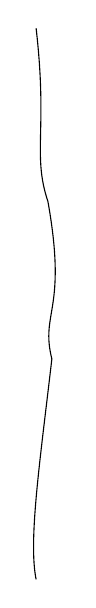
\begin{tikzpicture}[x=1cm,y=1cm]
\draw (0,7) .. controls (.15,5.7) and (-.05,5.4) .. (.15,4.8) .. controls (.4,3.4) and (.05,3.4) .. (.2,2.8) .. controls (.05,1.5) and (-.1,.5) .. (0,0);
\end{tikzpicture}}
